%-------------------------------------------------------------------------------
\section{Code performance}\label{sec:evaluation}
%-------------------------------------------------------------------------------
In the following, we illustrate the handling of \mf\ and the quality of the
resulting fits by means of several example spectra. In Section~\ref{sec:pwv},
the derivation of molecular abundances is discussed. In particular, the quality
of the derived water vapour column densities is investigated.
In Section~\ref{sec:tactest}, we briefly discuss the performance of \mf\ in
terms of the correction of telluric absorption features. Finally,
Section~\ref{sec:tips} provides some general rules that should be considered
for a successful application of \mf.

%-------------------------------------------------------------------------------
\subsection{Derivation of molecular abundances}\label{sec:pwv}
%-------------------------------------------------------------------------------
We illustrate the use of \mf\ for the derivation of molecular abundances by
means of a small sample of spectra consisting of a CRIRES, an X-Shooter, and
a pair of VISIR spectra (see Table~\ref{tab:sample}). The high-resolution
($R \approx 50000$) CRIRES standard star spectrum is typical of spectra that
are used for the nocturnal \ac{PWV} measurements at the VLT \cite{PWV}. Despite
of the narrow wavelength range from 3.274 to 3.352\,$\mu$m, the good resolution
allows one to fit many individual telluric absorption lines, which usually
results in convincing fits of the water vapour content and abundances of other
significant molecules in the atmosphere. The medium-resolution
($R \approx 8800$) X-Shooter VIS-arm star spectrum demonstrates \cite{PWV}
measurements in a narrow wavelength range at relatively short wavelengths
(0.940 to 0.951\,$\mu$m). Finally, the VISIR LR-mode spectra
($R \sim$ a few hundred) are examples for sky radiance spectra in the mid-IR
that are dominated by water vapour emission (see Section~\ref{sec:spectra}).
Since the very low resolution is not optimal for deriving \ac{PWV} values,
these spectra can be used to test the limits of the method. The presence of
spectra that were taken at similar time but for different wavelength regimes
allows some interesting comparisons.

\begin{table*}
\caption[]{Description of test sample}
\label{tab:sample}
\centering
\vspace{5pt}
\begin{tabular}{l l l l c c c}
\hline\hline
\noalign{\smallskip}
Label & Inst. & T/R$^\mathrm{a}$ & Resolution &
$\lambda^\mathrm{b}$ [$\mu$m] & Date & Time [UT] \\
\noalign{\smallskip}
\hline
\noalign{\smallskip}
C1 & CRIRES & T & high & $3.274 - 3.352$ & 2008/07/26 & 02:50 \\
V1 & VISIR & R & low & $10.37 - 12.50$ & 2009/10/25 & 04:07 \\
V2 & VISIR & R & low & $11.17 - 13.30$ & 2009/10/25 & 04:26 \\
X1 & X-Shooter & T & medium & $0.53 - 1.02$ & 2010/11/16 & 06:49 \\
\noalign{\smallskip}
\hline
\end{tabular}
\begin{list}{}{}
\item[$^\mathrm{a}$] transmission or radiance.
\item[$^\mathrm{b}$] The full wavelength range is shown. This is also the fit
range except for X1, which was fitted in the two ranges $0.762 - 0.770$\,$\mu$m
(part of the O$_2$ A-band) and $0.940 - 0.951$\,$\mu$m (H$_2$O absorption).
\end{list}
\end{table*}

\begin{table*}
\caption[]{\ac{PWV} results for the test sample in Table~\ref{tab:sample}}
\label{tab:results}
\centering
\vspace{5pt}
\begin{tabular}{l l c c c c c c}
\hline\hline
\noalign{\smallskip}
Label & Fit molecules$^\mathrm{a}$ & $t_\mathrm{fit}$ [min]$^\mathrm{b}$ &
\multicolumn{2}{c}{H$_2$O column [mm]} & PWV$_\mathrm{fit}$/ & rel. RMS \\
& & & ESO$^\mathrm{c}$ & {\tt molecfit} & PWV$_\mathrm{init}$$^\mathrm{d}$ & [\%] \\
\noalign{\smallskip}
\hline
\noalign{\smallskip}
C1 & H$_2$O, O$_3$, CH$_4$ &  1.2 & 0.89 & 0.99 & 0.885 & 2.0 \\
V1 & H$_2$O, CO$_2$, O$_3$ & 17.3 & 2.25 & 2.55 & 1.291 & 5.7 \\
V2 & H$_2$O, CO$_2$, O$_3$ & 16.8 & 2.25 & 1.87 & 0.982 & 9.0 \\
X1 & H$_2$O, O$_2$         &  0.6 & 0.96 & 0.92 & 0.605 & 4.1 \\
\noalign{\smallskip}
\hline
\end{tabular}
\begin{list}{}{}
\item[$^\mathrm{a}$] VISIR: CO$_2$ and O$_3$ calculated but not fitted; fixed
{\sc relcol}: CO$_2$: 1.06 (390\,ppmv; global reference value for 2011
\cite{CDIAC}), O$_3$: 1.08 (258 Dobson units; Patat et al. \cite{PAT11});
X-Shooter: O$_2$ calculated but not fitted ({\sc relcol} = 1)
\item[$^\mathrm{b}$] tested on a Core2Quad Q9550@2.83GHz, 8GB RAM, Fedora 16
(64 bit)
\item[$^\mathrm{c}$] CRIRES: taken from fit with the IDL {\tt molecgui} code
(A. Smette, ESO); VISIR: taken from the ESO \ac{PWV} monitor (VISIR but
different wavelength regime; closest measurement: $\Delta t \le 41$\,min);
X-Shooter: taken from ESO \ac{PWV} monitor (same spectrum, but measured in NIR
regime by means of a curve-of-growth analysis).
\item[$^\mathrm{d}$] ratio of the \ac{PWV} derived from best-fit and initial
atmospheric model.
\end{list}
\end{table*}

\begin{figure}
\centering
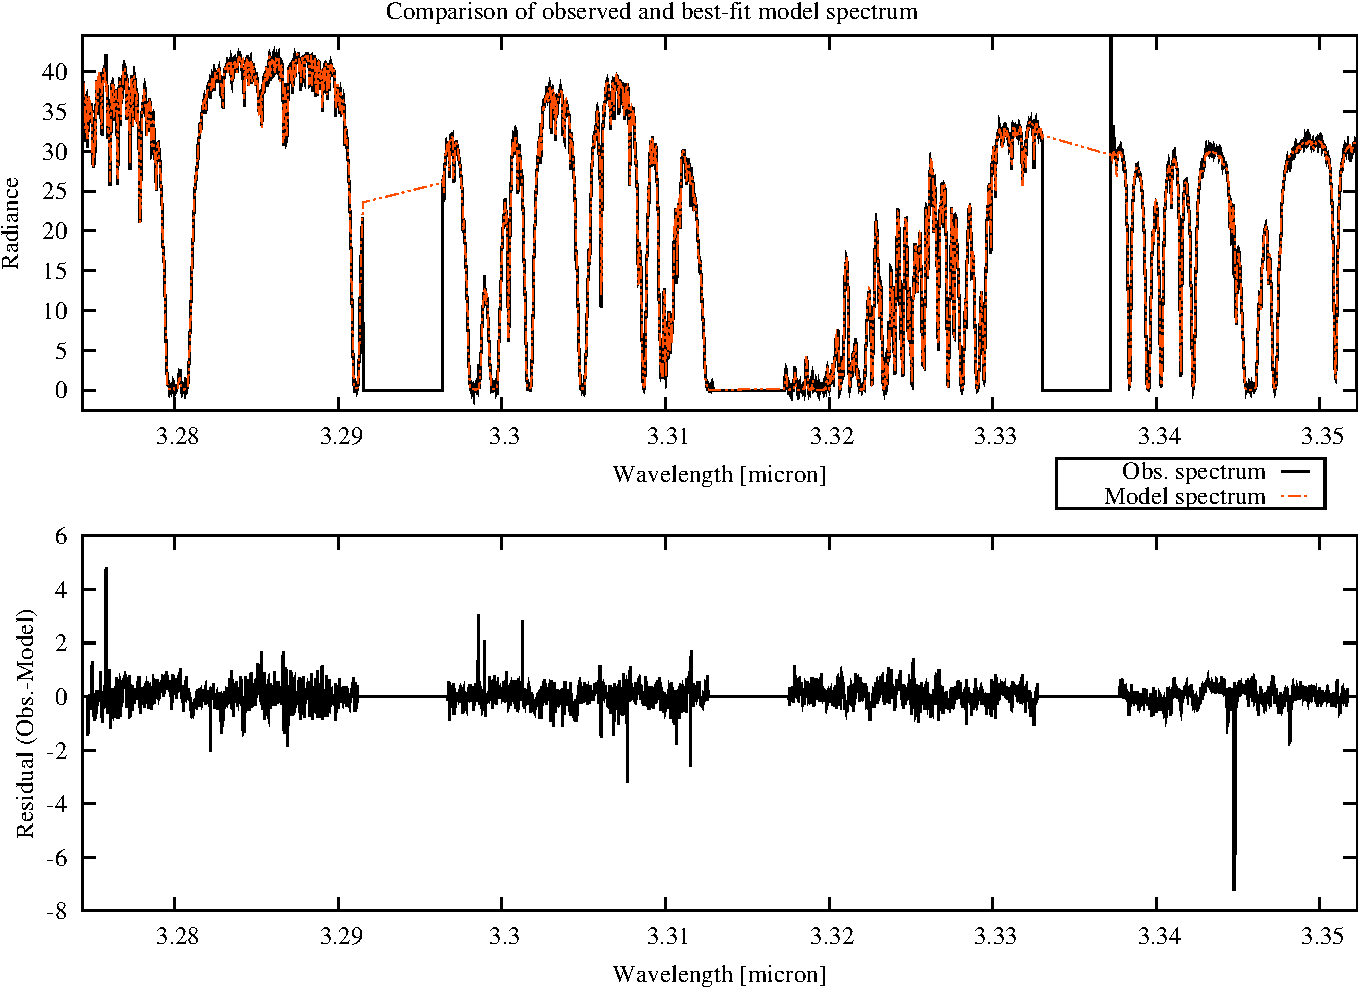
\includegraphics[width=0.7\textwidth,clip=true]
{figures/molecfit_crires_fit.pdf}
\caption[]{Comparison of the CRIRES spectrum C1 (black) and the best-fit model
(red). Wavelengths not covered by the four CRIRES chips are indicated by zero
radiance. The lower panel shows the difference of both spectra. Wavelengths
excluded from the fit are indicated by a residual of zero.}
\label{fig:crires}
\end{figure}

\begin{figure}
\centering
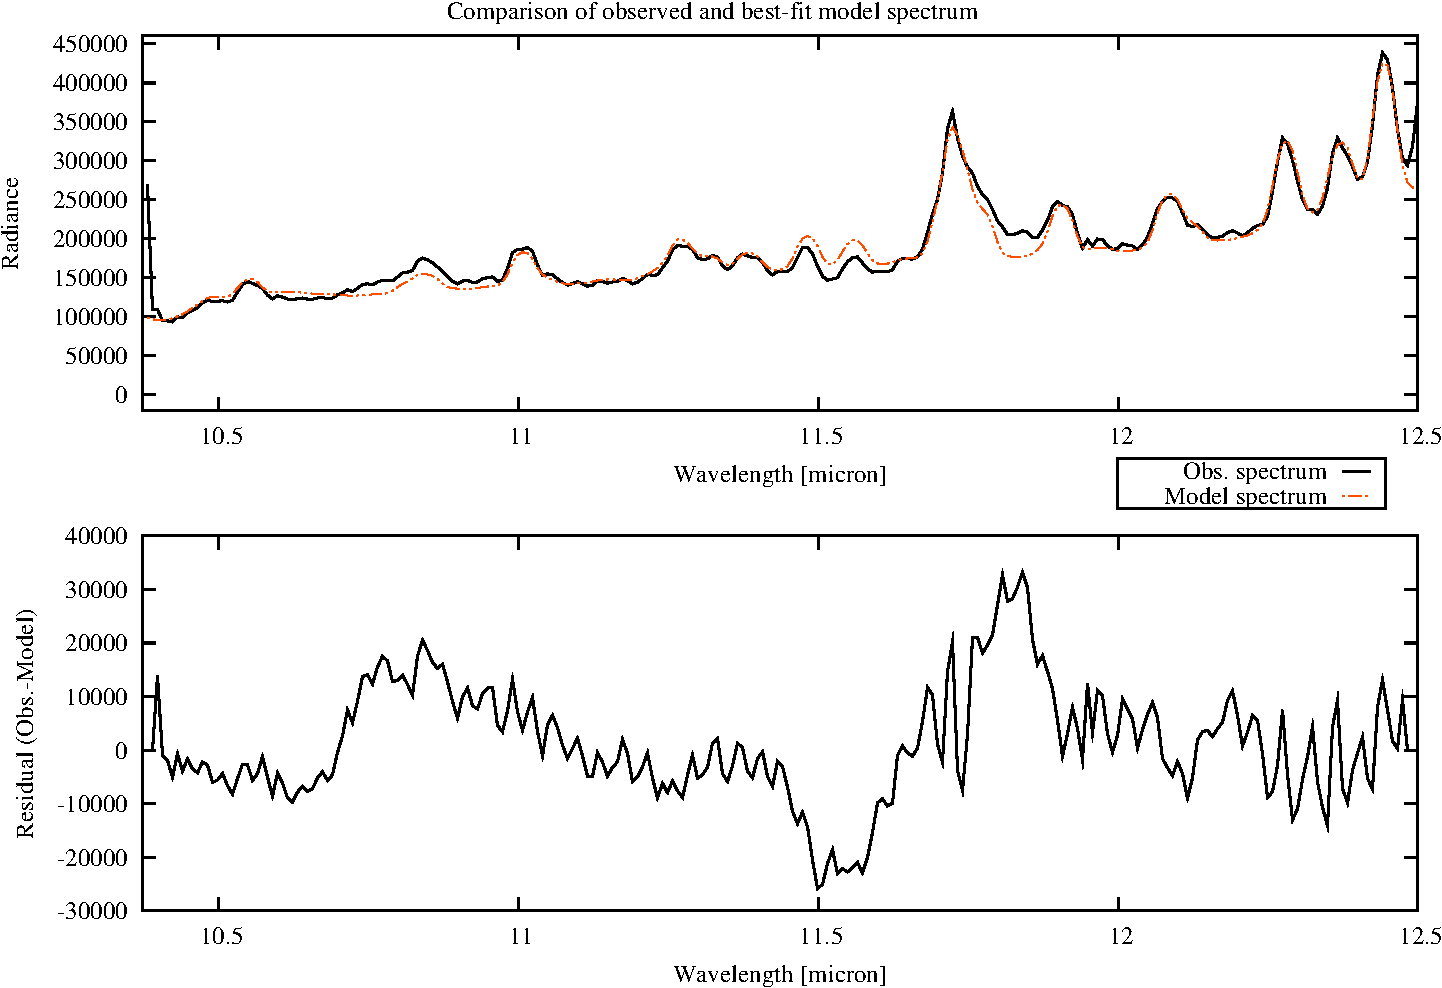
\includegraphics[width=0.7\textwidth,clip=true]
{figures/molecfit_VR_091024A_114_fit.pdf}
\caption[]{Comparison of VISIR spectrum V1 (black) and the best-fit model
(red). The lower panel shows the difference of both spectra.}
\label{fig:visir1}
\end{figure}

\begin{figure}
\centering
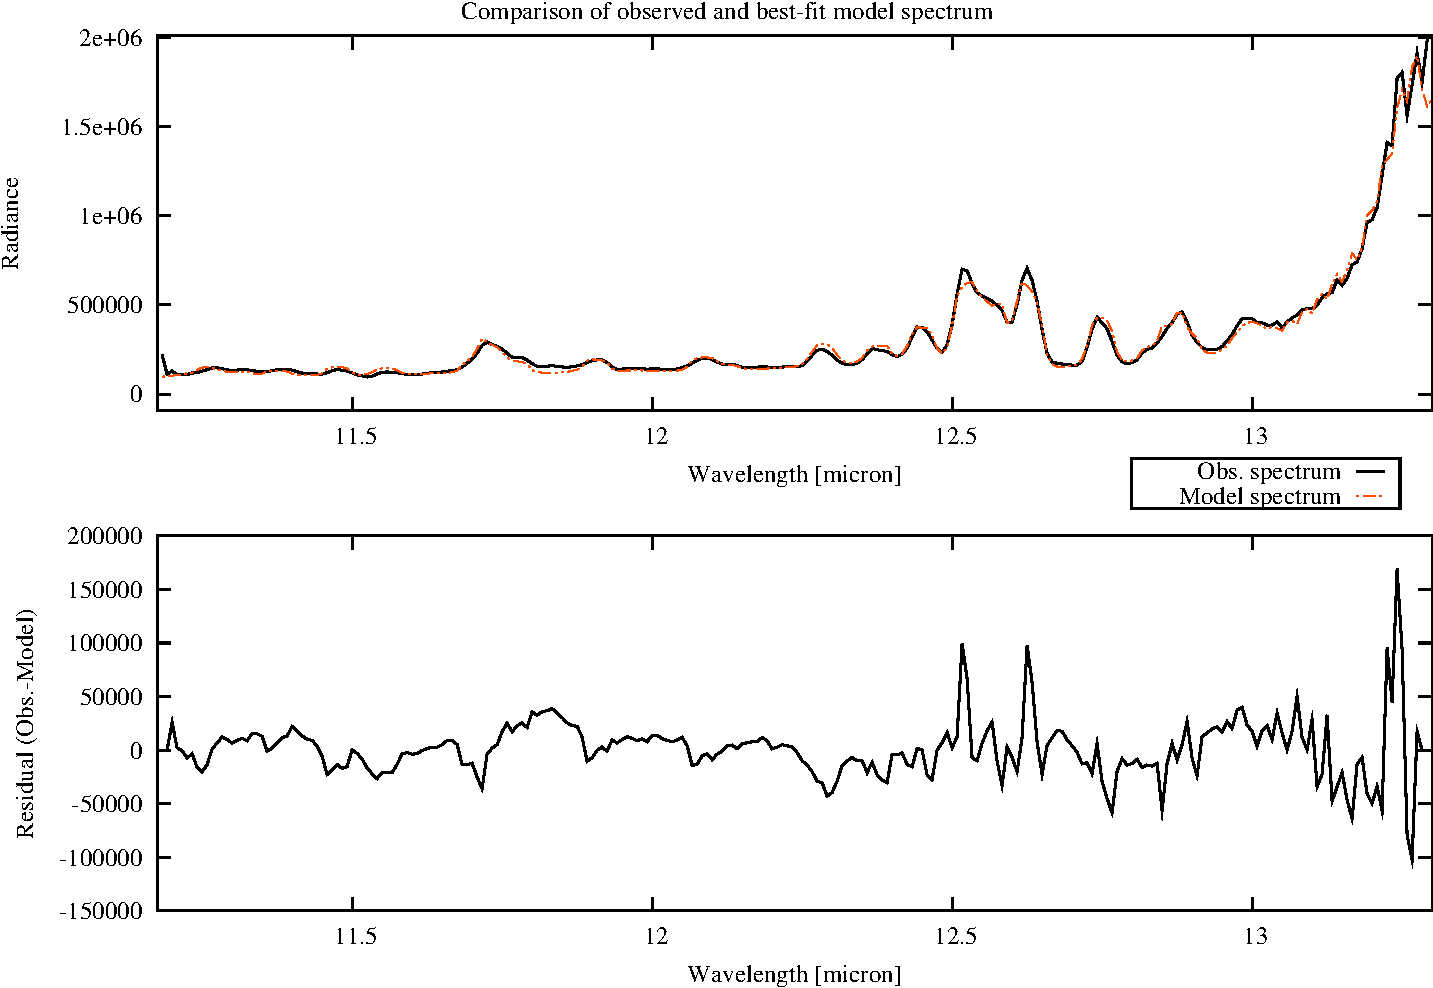
\includegraphics[width=0.7\textwidth,clip=true]
{figures/molecfit_VR_091024A_122_fit.pdf}
\caption[]{Comparison of VISIR spectrum V2 (black) and the best-fit model
(red). The lower panel shows the difference of both spectra.}
\label{fig:visir2}
\end{figure}

\begin{figure}
\centering
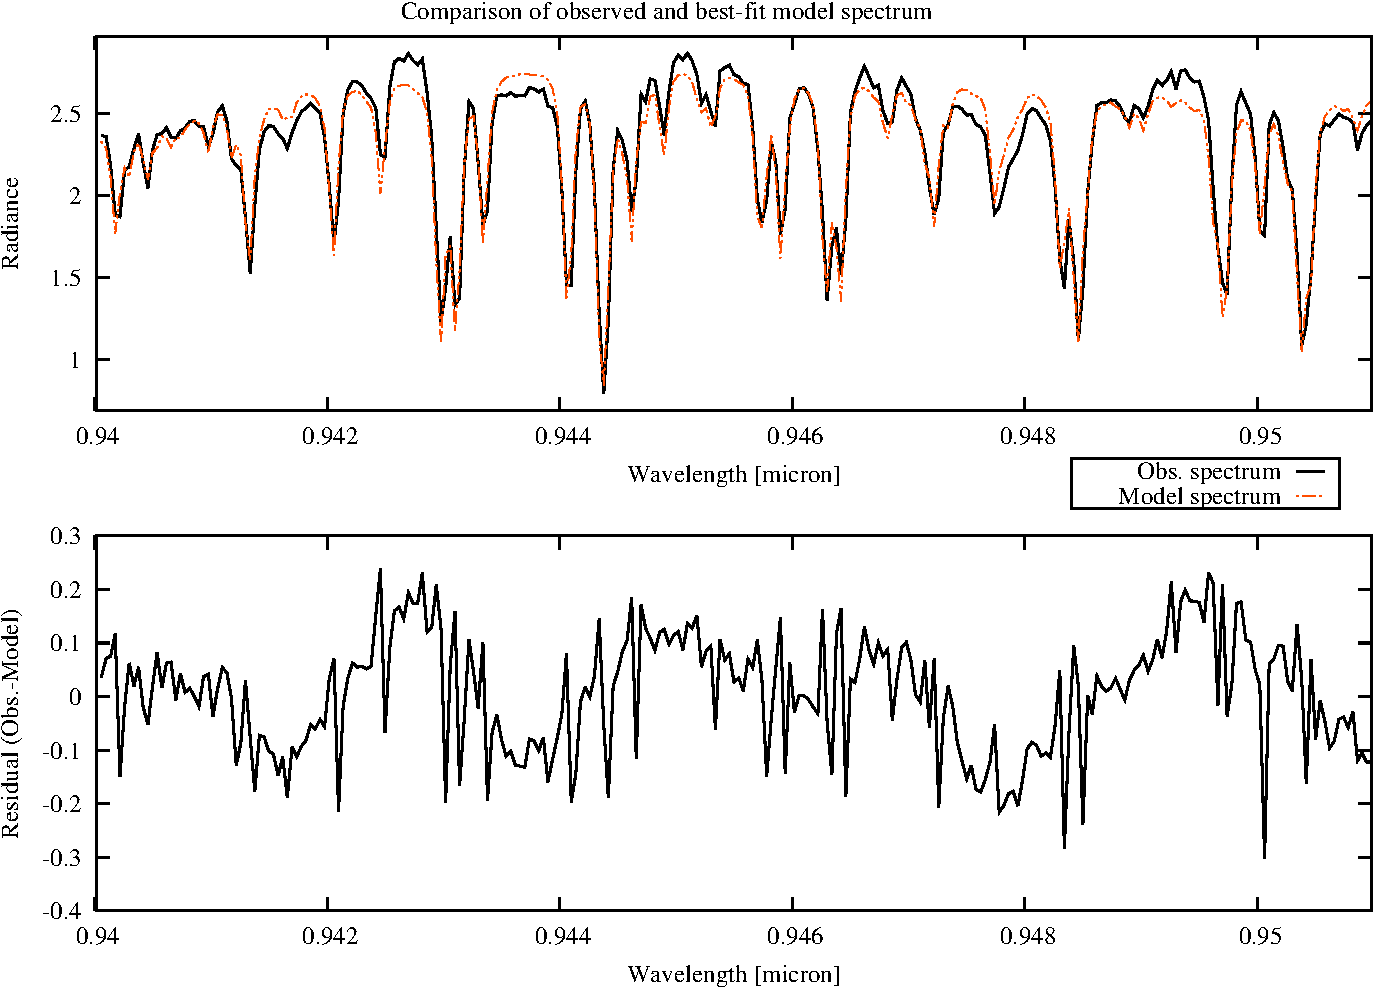
\includegraphics[width=0.7\textwidth,clip=true]
{figures/molecfit_xshoo_vis_1_fit_2.pdf}
\caption[]{Comparison of X-Shooter spectrum X1 (black) and the best-fit model
(red) for the fitted water vapour band. The lower panel shows the difference of
both spectra.}
\label{fig:xshooter}
\end{figure}

We evaluate \mf\ discussing a series of test runs for the sample of spectra
defined in Table~\ref{tab:sample}. For all sample spectra, the code was started
for a set of input parameters similar to those given in
Section~\ref{sec:paramfile}. By default, the spectra were fitted with
\ac{LBLRTM} and polynomials of degree 3 for the continuum and wavelength
correction. Due to a challenging continuum shape, a continuum polynomial of
degree 5 was chosen for spectrum V2. For X1, only a constant wavelength shift
was allowed because of the very narrow fit ranges compared to the full
spectrum (see Table~\ref{tab:sample}). The width and shape of the instrumental
function was partly constrained. While the width of the Gaussian was
unconstrained, the Lorentzian was fixed and the width was set to 0.5 pixels to
avoid a degenerated fit. Since this setting is somewhat arbitrary, the derived
\ac{PWV} values could be offset compared to the real ones. In particular, this
could be true for X-Shooter spectra, for which a significant Lorentzian
component could not be detected, so far. Tests indicate uncertainties in the
order of 0.1\,mm. Due to the relatively small number of pixels in the fit
range, the Gaussian/Lorentzian kernel radius of the X-Shooter and VISIR spectra
was reduced from 300\,FWHM for CRIRES to 30\,FWHM. A boxcar was only fitted for
the VISIR sky radiance spectra. Moreover, the VISIR fits were carried out with
an initial emissivity of $0.1$. For the fitting, the wavelength ranges provided
in Table~\ref{tab:sample} were used, except for a few pixels at the edges
(20/40 pixels for CRIRES, 3 pixels for VISIR). The selection of the fit
molecules depended on the fit wavelength range. 1 to 3 molecules of H$_2$O,
CO$_2$, O$_3$, and CH$_4$ were considered for a fit (see
Section~\ref{sec:spectra} for an explanation). Since the fit ranges of the
VISIR spectra were optimised for water-related features (see
Table~\ref{tab:sample}), the abundances of the minor contributions CO$_2$ and
O$_3$ were fixed and set to reasonable values. The selected molecules and the
fit results are summarised in Table~\ref{tab:results}. Figures~\ref{fig:crires}
to \ref{fig:xshooter} show examples for comparisons of observed input spectra
and best-fit models. The plots were created by \mf. It should be noted that the
setups were not tuned to provide the best possible fits, which might explain at
least some of the fitting discrepancies.

As indicated by Table~\ref{tab:results}, the six test spectra are well fitted.
The RMS relative to the mean flux ranges from 2\% for the CRIRES spectrum to
9\% for the redder VISIR spectrum V2. The strongest residual in
Figure~\ref{fig:crires} is caused by a stellar line, which was not masked due
to its negligible contribution to the global fit. In Figure~\ref{fig:visir2},
the strong emission at the red end of the spectrum is caused by CO$_2$. For
this reason, spectrum V2 is less well suited for water vapour fitting than the
spectrum V1 at shorter wavelengths. The fitting times are very different for
the four setups. They depend on the width of the wavelength range and number of
lines to be calculated by \ac{LBLRTM}. For this reason, the fit of the
X-Shooter spectrum just took 36\,s. Note that the long code run times for the
VISIR spectra could be significantly reduced if the basic (now outdated)
\ac{HITRAN}~2008 line list was used instead of the more complex {\tt aer} line
list (see Section~\ref{sec:molecs} and Appendix~\ref{app:linelist}). The
derived \ac{PWV} values range from 0.92 to 2.55\,mm. These values can be
compared to those derived with different approaches and/or different spectra.
Table~\ref{tab:results} shows good agreement of the \mf\ results and data taken
from the ESO \ac{PWV} monitor \cite{PWV}. Typical deviations are
in the order of 0.1\,mm for the high resolution data, which agrees well with
the reported uncertainties of the \ac{PWV} monitor fits. Test data fits with
different parameter sets suggest \ac{PWV} errors in the same range for \mf.
For the VISIR data, the deviations are significantly higher. The direct
comparison of the results for the two VISIR spectra confirms that these setups
are not well suited for water vapour fits. On the other hand, the RMS values
are convincing, which suggests that the fits of the low resolution VISIR
spectra suffer from degeneracies. \ac{PWV} measurements of distinctly higher
quality can be expected for data like the CRIRES spectrum with many deep and
narrow absorptions.

A reliable \ac{PWV} measurement does not imply that all fit parameters are
trustworthy. In particular, abundances of molecules without sufficiently strong
spectral features and parameters for the adaptation of the model spectrum
to the observed spectrum such as continuum, wavelength, and resolution
parameters (see Section~\ref{sec:adaption}) are affected if the fitting problem
is degenerated. An example is the convolution kernel, where the relative
contributions of boxcar, Gaussian, and Lorentzian are difficult to determine.
Another example is the telescope emissivity (see Section~\ref{sec:greybody}),
which is a fit parameter for sky radiance spectra. Values of 0.079 (V1) and
0.039 (V2) for the VISIR spectra show a significantly higher uncertainty than
the \ac{PWV} measurements. This implies that the H$_2$O abundance is a
relatively robust fit parameter and that there are parameters which require
significantly higher quality data.

Table~\ref{tab:results} also includes the ratio of the best-fit \ac{PWV} and
the \ac{PWV} derived from the initial parameters. Since the initial H$_2$O
profile is derived from an atmospheric standard profile, a suitable
meteorological \ac{GDAS} model profile, and ground-based meteorological data
from the \ac{EMM} (see Section~\ref{sec:profiles}), the derived \ac{PWV} ratios
can be used to estimate the quality of this profile-composition procedure,
provided that the radiative transfer code produce realistic molecular spectra.
A wide range of ratios between $0.605$ and $1.291$ was found, which indicates
that the input profiles can lead to a significantly under- or overestimated
atmospheric water content. This result shows the importance of the fitting
procedure for obtaining realistic \ac{PWV} values. The effect of the input
water vapour profile on the fit quality is extensively discussed in the
SM-03 Science Report \cite{SM03SR}.

%-------------------------------------------------------------------------------
\subsection{Telluric absorption correction}\label{sec:tactest}
%-------------------------------------------------------------------------------
Apart from deriving abundances of greenhouse gases, \mf\ is designed to
be used for the correction of telluric absorption features. For this
purpose, the routine {\tt calctrans} provides the best-fit model transmission
(see Section~\ref{sec:algorithm}). It also corrects the fitted spectrum.

{\tt calctrans\_lblrtm} and {\tt calctrans\_convolution} provide the best-fit
model transmission and perform the convolution of the spectrum separately.

\sloppy For
correcting other spectra taken under similar atmospheric conditions and
airmasses, the executable {\tt corrfilelist} can be used. In the following, we
briefly discuss telluric absorption correction for CRIRES
(Section~\ref{sec:crires}) and X-Shooter spectra (Section~\ref{sec:xshooter}).

%-------------------------------------------------------------------------------
\subsubsection{CRIRES}\label{sec:crires}
%-------------------------------------------------------------------------------
\begin{table*}
\caption[]{Description of data and results for the CRIRES telluric absorption
correction test}
\label{tab:tactest}
\centering
\vspace{5pt}
\begin{tabular}{c c c c c c c}
\hline\hline
\noalign{\smallskip}
Pair & Target$^\mathrm{a}$ & Time$^\mathrm{b}$ [UT] & Airmass & PWV [mm] &
rel. RMS$^\mathrm{c}$ [\%] & Model RMS$^\mathrm{d}$ [\%] \\
\noalign{\smallskip}
\hline
\noalign{\smallskip}
1 & T & 2:49 & 1.569 & 0.83 & 3.6 & 0.9 \\
1 & S & 3:08 & 1.546 & 0.90 & 2.0 &     \\
2 & T & 3:58 & 1.472 & 0.86 & 3.4 & 1.0 \\
2 & S & 4:19 & 1.475 & 0.92 & 2.1 &     \\
\noalign{\smallskip}
\hline
\end{tabular}
\begin{list}{}{}
\item[$^\mathrm{a}$] T = telluric standard star, S = science object
\item[$^\mathrm{b}$] All spectra were taken on July 30th, 2009.
\item[$^\mathrm{c}$] deviation of best-fit model from observed spectrum;
relative to mean flux
\item[$^\mathrm{d}$] deviation of model transmission curve for telluric star
from corresponding model for science spectrum; absolute value
\end{list}
\end{table*}

\begin{figure}
\centering
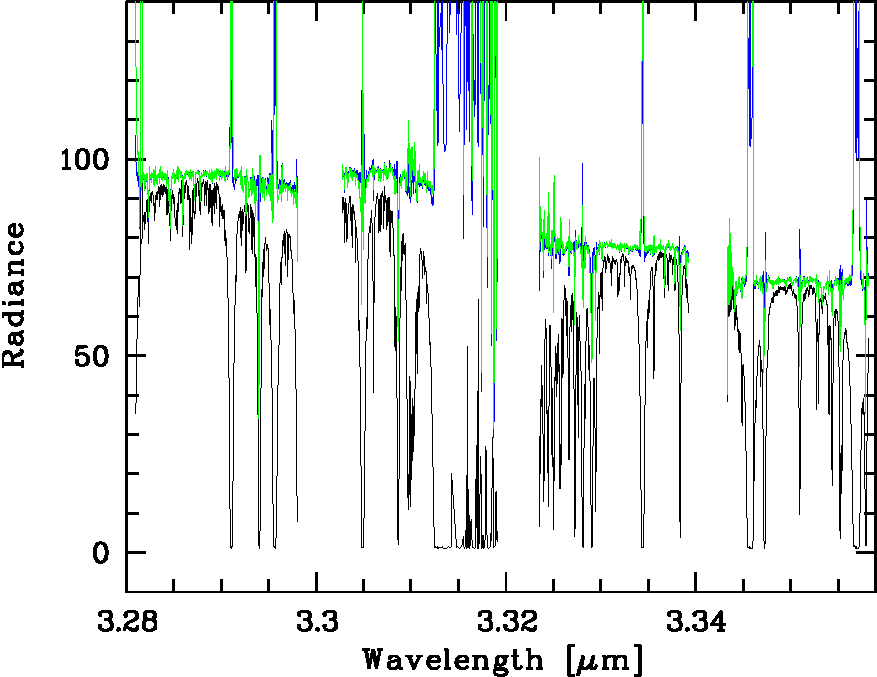
\includegraphics[width=0.7\textwidth,clip=true]
{figures/mfd_tactest1.pdf}
\caption[]{Correction of telluric absorption features in science spectrum 1
(black). The blue and the green curves display the corrected spectra obtained
by transmission models fitted to the science and the telluric standard star
spectra. No data is shown for wavelengths suffering from very high atmospheric
opacity (radiance lower than 1 unit).}
\label{fig:tactest1}
\end{figure}

\begin{figure}
\centering
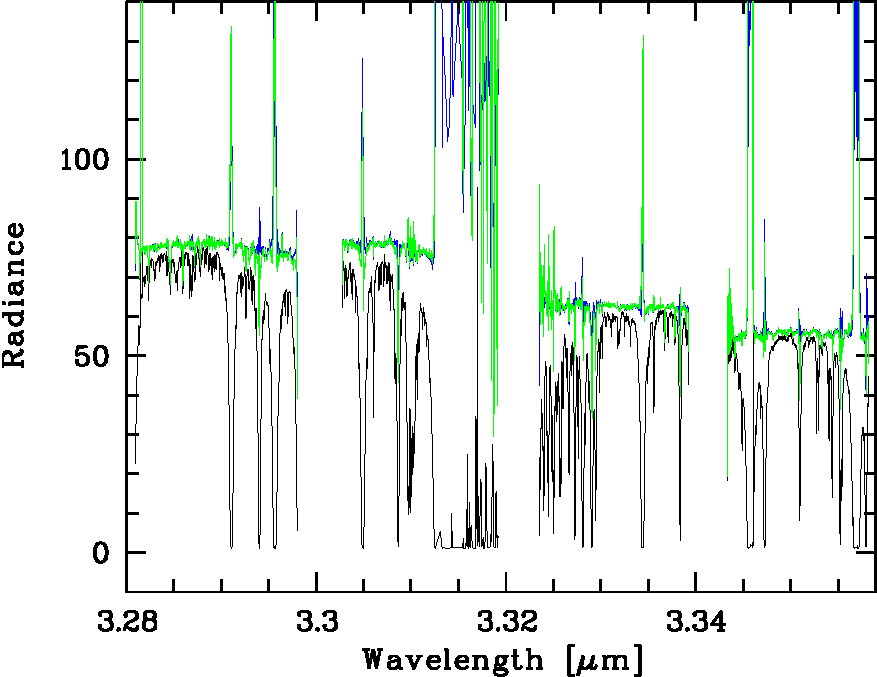
\includegraphics[width=0.7\textwidth,clip=true]
{figures/mfd_tactest2.pdf}
\caption[]{Correction of telluric absorption features in science spectrum 2.
For details see Figure~\ref{fig:tactest1}.}
\label{fig:tactest2}
\end{figure}

In order to evaluate the performance of the code in terms of telluric feature
correction, we have studied two pairs of CRIRES observations in the wavelength
range from 3.28 to 3.36\,$\mu$m consisting of a telluric standard star spectrum
and a spectrum of a science target. The spectra of a pair were taken at almost
the same time and airmass (see Table~\ref{tab:tactest}). We run the code for
all spectra to obtain model transmission curves. The input parameters were set
as given in Section~\ref{sec:paramfile}. The resulting PWV values provided by
Table~\ref{tab:tactest} confirm that the spectra were taken at similar
atmospheric conditions. Moreover, these values suggest that the fits are
reliable, which is also indicated by RMS values relative to the mean flux
between 2.0 and 3.6\% (cf. Table~\ref{tab:results}).

The best-fit transmission curves as obtained for the standard stars and the
science targets were used to correct the spectra of the science targets. The
resulting spectra are displayed in Figures~\ref{fig:tactest1} and
\ref{fig:tactest2}. Except for wavelengths suffering from very low transmission
and strong transmission gradients, the corrected spectra show only weak line
residuals. In general, the correction appears to be satisfying for transmission
fractions greater than 70 to 80\%. The large errors for the centres of
optically thick lines can be explained by the division by very small numbers
and small errors by statistical noise and in the zero flux line of the observed
spectra. Small errors in the wavelength grid and line profile fit cause
residuals in the wings of the lines. Interestingly enough, the correction of a
science spectrum by a fit of this spectrum itself is not worse than the result
based on the standard star transmission curve. The similarity in the correction
functions is also indicated by the very small RMS values of about 1\% given in
Table~\ref{tab:tactest}. Hence, the test data set could be corrected without
the need of telluric standard star observations. However, it is not clear
whether this is also true for spectra taken at a different time, other science
targets, and other instrumental setups. Moreover, a systematic comparison with
the results of classical methods of telluric absorption correction is missing.
This is out of the scope of this document and will be discussed elsewhere.

%-------------------------------------------------------------------------------
\subsubsection{X-Shooter}\label{sec:xshooter}
%-------------------------------------------------------------------------------
For X-Shooter, an investigation of a large data set was carried out, which is
summarised in the SM-03 Science Report \cite{SM03SR}. In this document, we
focus on the illustration of the telluric absorption correction for an example
NIR-arm X-Shooter spectrum. The flux-calibrated 1D spectrum was obtained by the
ESO X-Shooter standard pipeline (see Modigliani et al. \cite{MOD10}). It was
provided to \mf\ as FITS image. See section \ref{sec:inputspec} for more
information about the Molecfit input spectrum format.

\begin{table*}
\caption[]{Fit ranges for the example X-Shooter NIR-arm spectrum}
\label{tab:fitranges}
\centering
\vspace{5pt}
\begin{tabular}{c c c}
\hline\hline
\noalign{\smallskip}
ID & Range [$\mu$m] & Molecule \\
\noalign{\smallskip}
\hline
\noalign{\smallskip}
1 & $1.12 - 1.13$ & H$_2$O \\
2 & $1.47 - 1.48$ & H$_2$O \\
3 & $1.80 - 1.81$ & H$_2$O \\
4 & $2.06 - 2.07$ & CO$_2$ \\
5 & $2.35 - 2.36$ & CH$_4$ \\
\noalign{\smallskip}
\hline
\end{tabular}
\end{table*}

\begin{figure}
\centering
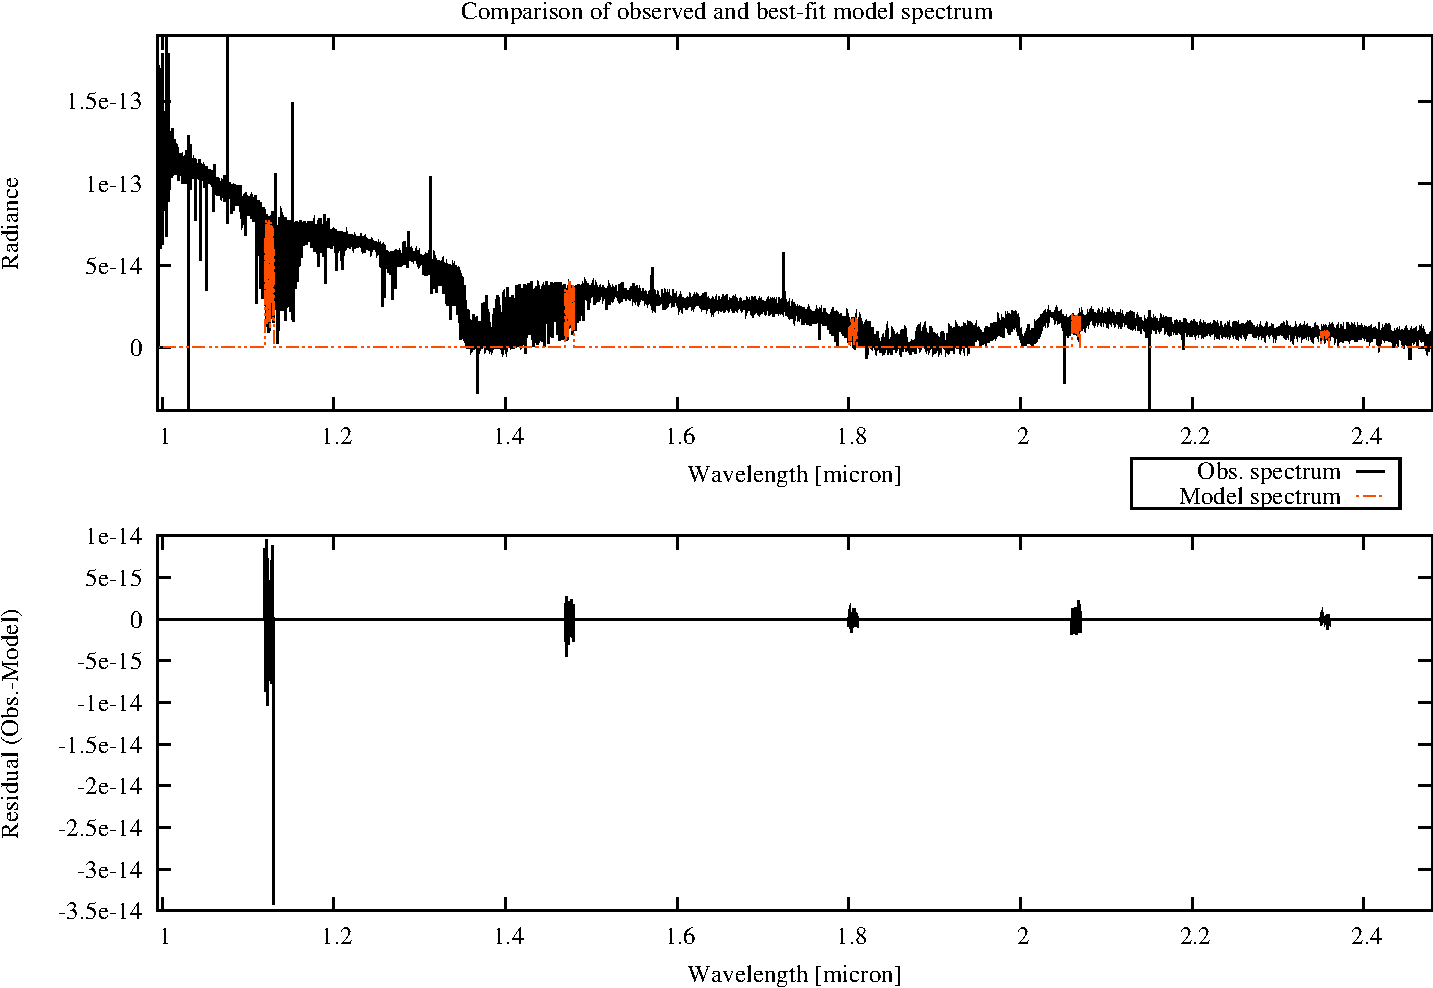
\includegraphics[width=0.7\textwidth,clip=true]
{figures/molecfit_xshoo_tellstd_nir_fit.pdf}
\caption[]{Comparison of a NIR-arm X-Shooter spectrum of a telluric standard
star (black) and the best-fit model (red) for five fit ranges of 10\,nm in
size. The lower panel shows the difference of both spectra. Wavelengths
excluded from the fit are indicated by zero transmission in the upper panel
and a residual of zero in the lower panel.}
\label{fig:xsh_fit}
\end{figure}

\begin{figure}
\centering
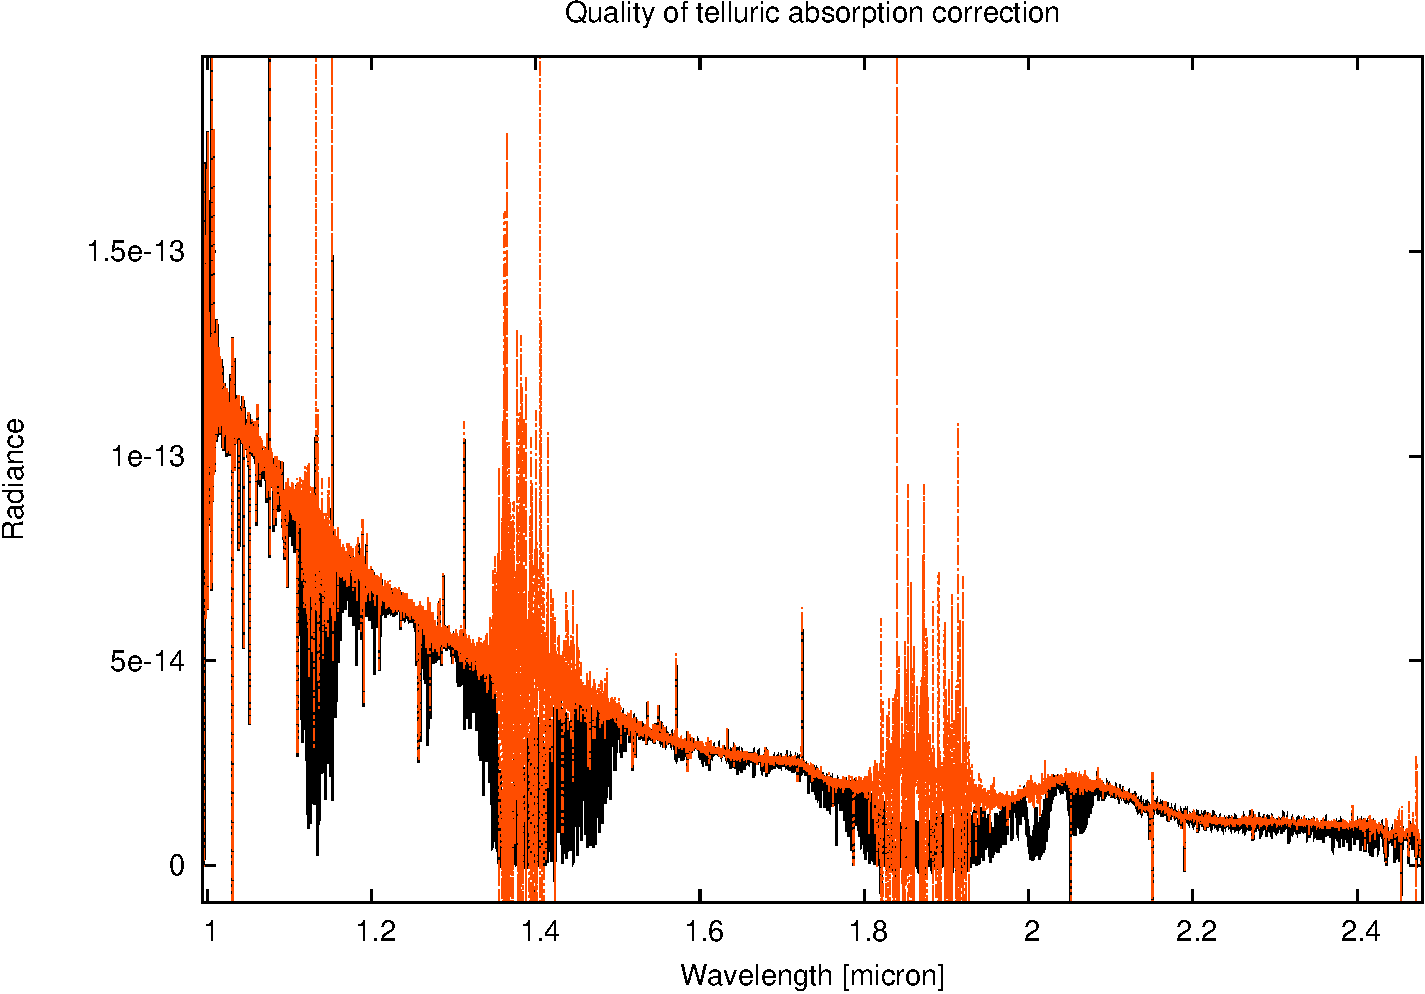
\includegraphics[width=0.7\textwidth,clip=true]
{figures/molecfit_xshoo_tellstd_nir_tac.pdf}
\caption[]{Comparison of a NIR-arm X-Shooter spectrum of a telluric standard
star (black) and the same spectrum corrected for telluric absorption based on
the fit shown in Figure~\ref{fig:xsh_fit} (red).}
\label{fig:xsh_tac}
\end{figure}

For the fitting, we used a similar parameter setup as described in
Section~\ref{sec:pwv} for the X-Shooter VIS-arm spectrum. However, there are
some important differences. Since the telluric feature correction has to be
carried out for the entire spectrum ranging from 0.99 to 2.48\,$\mu$m, we have
defined five narrow fit ranges in different parts of the spectrum, which are
listed in Table~\ref{tab:fitranges}. Each range of 10\,nm in size comprises 100
pixels. The low coverage of the spectrum by fit ranges (about 3\% of the full
spectrum) is necessary to obtain \mf\ results within a few minutes. Tests
indicate that this limitation does not significantly deteriorate the correction
compared with runs using more windows. The fit ranges cover lines from H$_2$O,
CO$_2$, and CH$_4$ (see Table~\ref{tab:fitranges}). However, we only fit the
strongly varying water vapour lines. For the other molecules and O$_2$ and
CO, which also have lines in the near-IR regime, we use the abundances from
the atmospheric standard profile (see Section~\ref{sec:mipas}). In the case of
CO$_2$, we used a {\sc relcol} value of 1.06 instead of 1 (see
Section~\ref{sec:params}) in order to take into account the global increase in
CO$_2$ during the last decade. The use of fixed molecular column densities for
all molecules but H$_2$O makes the fit more robust and faster. The low
variability of the fixed species does not significantly affect the quality of
the telluric absorption correction (see below). Another measure to stabilise
the fit is the restriction to wavelength shifts, \ie\ the neglection of higher
order Chebyshev polynomials for the wavelength correction (see
Section~\ref{sec:wavegrid}). Moreover, the continuum correction was limited to
wavelength-independent factors for each fit range. Since the fit ranges are
very narrow, it is a good assumption that the variation of the stellar
continuum (strong stellar lines are not present) is significantly lower than
the variation of the telluric absorption. As general start value
$1 \times 10^{-13}$ was chosen to avoid changes of the continuum parameter by
many orders of magnitude in the course of the fitting procedure. Finally,
X-Shooter spectra show a nearly linear increase of the line widths with
increasing wavelength. We considered this correlation for the convolution
kernel calculation by using the {\sc varkern}~=~1 option (see
Section~\ref{sec:params}).

Figures~\ref{fig:xsh_fit} and \ref{fig:xsh_tac} show the results of the fitting
procedure and the telluric absorption correction. The figures were created by
\mf\ and {\tt calctrans} respectively. Figure~\ref{fig:xsh_fit} illustrates
the position of the fit ranges and shows the fit residuals. The relative RMS
amounts to relatively low 4.2\%. Further results of the fit are an intermediate
\ac{PWV} value of 2.4\,mm, a moderate average wavelength shift of 0.35~pixels
of the observed spectrum towards shorter wavelengths, and a best-fitting
Gaussian kernel FWHM of 1.2~pixels for a fixed Lorentzian of 0.5~pixels. As
Figure~\ref{fig:xsh_tac} demonstrates, the fit parameters derived from the
five narrow windows are also suitable to correct the full spectrum for telluric
absorption. Down to transmission values of less than 0.5, the residuals are
relatively small in general. This is particularly true for the CO$_2$ bands at
about 2\,$\mu$m. Consequently, the assumed fixed CO$_2$ concentration has
turned out to be correct. For very low transmissions close to 0, the residuals
are significantly increasing. However, this effect is expected, since the
correction in these ranges corresponds to the division of two very small
numbers, which are affected by strong relative statistical and systematical
errors. For this reason, the results for the cores of the H$_2$O bands between
the $J$, $H$, and $K$ bands have to be taken with care. It is expected that the
near-IR spectrum of a hot telluric standard star is monotonic decreasing.
However, the corrected spectrum shows bumps and troughs in regions of low
atmospheric transmission. This is most probably caused by a poor flux
calibration, since the removal of the bumps related to the H$_2$O bands would
require an unrealistic water vapour reduction of about 40\%. For this reason, a
simple interpolation between regions of high transmission must fail in the
discussed near-IR wavelength ranges. For improving the pipeline performance in
future, the \mf\ results are very promising, since they show that the
wavelength regions with reliable continuum can be extended significantly.

%-------------------------------------------------------------------------------
\subsection{Tips and tricks}\label{sec:tips}
%-------------------------------------------------------------------------------
In the following, we provide a summary of rules that should be taken into
account for a successful application of \mf:
\begin{itemize}
\item Pixels with possible defects that could affect the fit quality can be
excluded from the fit in two ways. First, the critical pixels can be listed
in an ASCII or FITS file that is provided by the parameter
{\sc prange\_exclude} (see Section~\ref{sec:params}). Second, pixels can be
skipped by adding a mask column to an input ASCII or FITS table, or adding an
mask extension to a FITS image. In both cases, the name of the column/extension
has to be given by the fourth {\sc columns} parameter.
\item The resulting best-fit parameters of \mf\ are written to a {\tt .res}
file (see Section~\ref{sec:resfile}). In the case of a complex fit, the more
reliable fit parameters could be taken from this file and used as (fixed) input
for another iteration of the fitting procedure.
\item Changing the fit parameters {\sc ftol} and {\sc xtol} (see
Section~\ref{sec:params}) can significantly affect the code run time and the
quality of the fit. In the case of unsatisfying fit results, it may be an
option to change the default values. However, the effect is often
unpredictable, since more relaxed convergence criteria can lead to worse as
well as better fit quality.
\item To achieve an optimal performance of the code, one should fit only those
molecules that significantly contribute to the wavelength range of the fit. We
suggest to base the selection of relevant molecules on the information given in
Section~\ref{sec:spectra}.
\item In principle, PWV values can be measured by means of all kinds of spectra
of bright standard stars which show telluric lines in absorption and
atmospheric emission spectra in the thermal IR. However, a good fit requires
significant H$_2$O features. This criterion cannot be fulfilled if the water
lines are very weak as in the optical. Moreover, too low resolution can smooth
out the crucial lines, which can make the fit very unstable or even impossible
(see Section~\ref{sec:pwv}).
\item For \mf\ applications aiming at the derivation of the atmospheric water
vapour content or the telluric absorption correction of astronomical spectra,
it is often sufficient to set the abundances of other molecules to a fixed
value. For the more frequent molecules in the atmosphere (see
Section~\ref{sec:spectra}), the column density from the input standard profile,
\ie\ {\sc relcol}~=~1, is usually relatively close to the true value. It has
to be taken into account that the MIPAS standard profiles were created in 2001
(see Section~\ref{sec:mipas}), which causes deviations for greenhouse gases
that indicate a significant long-term increase in atmospheric abundance. For
example, the global CO$_2$ concentration increased by about 6\% in one decade,
which suggests {\sc relcol}~=~1.06 (see Section~\ref{sec:pwv}).
\item The user can explicitly set the initial value of the constant term of
the polynomials for the continuum correction and the wavelength solution. The
higher-order coefficients are automatically set to reasonable start values if
required (see Section~\ref{sec:params}). Setting {\sc wlc\_const} is only
recommended if a wavelength shift towards a certain direction is expected. The
{\sc cont\_const} is more critical. If the continuum level of the input
spectrum strongly deviates from 1, even after setting the scaling factor
{\sc flux\_unit} (see Section~\ref{sec:params}), it is prudent to adapt this
term.
\item For a correct wavelength fit especially at high resolution, it is
important to have a correct setting of the {\sc vac\_air} parameter. The
wavelength system depends on the instrument and the wavelength calibration
approach by the data reduction pipeline. IR data (CRIRES, VISIR) tend to be
provided in vacuum wavelengths, whereas data at shorter wavelengths tend to
be provided in air wavelengths (X-Shooter). If the user does not know this
necessary input, it can be easily derived by running \mf\ with both
{\sc vac\_air} options.
\item For the instrumental profile created by the convolution of boxcar,
Gaussian, and Lorentzian kernels (see Section~\ref{sec:adaption}), a derivation
from the fit can be difficult. If the $\chi^2$ degeneration by the kernel
parameters cause a bad fit, we recommend to modify the initial values of these
parameters or to fix the width of a kernel element. Some knowledge on the true
functional form of the instrumental profile can be quite helpful. For a first
test, the width of the Lorentzian might be fixed. For CRIRES, a value of 0.75
plus a large kernel size could be reasonable (A. Smette 2012, priv. comm.).
For our tests, we used 0.5 pixels for all instruments (see
Sections~\ref{sec:pwv} and \ref{sec:tactest}), although X-Shooter spectra do
not indicate a significant contribution of a Lorentzian. The boxcar kernel can
probably be neglected if the slit width does not have a significant impact on
the line FWHM. If the user has access to a suitable line profile kernel, it
can be imported via the parameter {\sc kernel\_file} (see
Section~\ref{sec:resolution}). The three-component profile fitting is switched
off in this case.
\item The run time of the radiative transfer code LBLRTM depends on the
width of the fitted wavelength ranges. For a better performance, it is,
therefore, recommended to use fit ranges as narrow as possible. It also makes
the polynomial continuum fit more reliable. For \eg\ X-Shooter, several
representative ranges over the entire wavelength range covering lines of all
critical molecules could be defined. A suitable bin size is 10\,nm. CRIRES
spectra are sufficiently narrow that the full wavelength range can be used for
the fitting procedure.
\item For spectra covering a wide wavelength range and narrow fit ranges, the
degree of the polynomial for the wavelength solution {\sc wlc\_n} should be set
to 0 to avoid unpredictable wavelength corrections outside the fit ranges if
a telluric absorption correction is required. For X-Shooter, it is also
strongly recommended to set {\sc varkern}~=~1 in order to consider the change
of the instrumental profile with wavelength (see Section~\ref{sec:params}).
\item For telluric absorption correction in the thermal IR, it could be
advantageous to use the strong sky emission extracted as 1D spectrum as input
for \mf. {\tt calctrans} will then calculate the transmission function
belonging to the best-fit sky radiance spectrum. Finally, the object spectrum
can be corrected for telluric absorption via {\tt corrfilelist}.
\end{itemize}

